%----------------------------------------------------------------------------
\chapter{Overview of the Approach}
%----------------------------------------------------------------------------
In this chapter, the various aspects of the proposed approach are detailed. In Section \ref{sec_methodology}, the application of this methodology from the users' point of view: how are they meant to interact with the interactive automata learning framework - also called \textit{Interactive Learning Entity} or \textit{ILE} - and how they can utilize it to design reactive systems in a declarative way. Then, in Section \ref{sec_architecture}, the applied software architecture, software components, algorithms and data structures are presented in the following order: first, the components concerned with the automata learning algorithm, then those responsible for its interaction with the oracle component, then the possible interactions of the oracle with the engineer.
%----------------------------------------------------------------------------
\section{Overview of the Methodology} \label{sec_methodology}
%----------------------------------------------------------------------------
\begin{figure}[!ht] 
	\centering
	\fbox{
		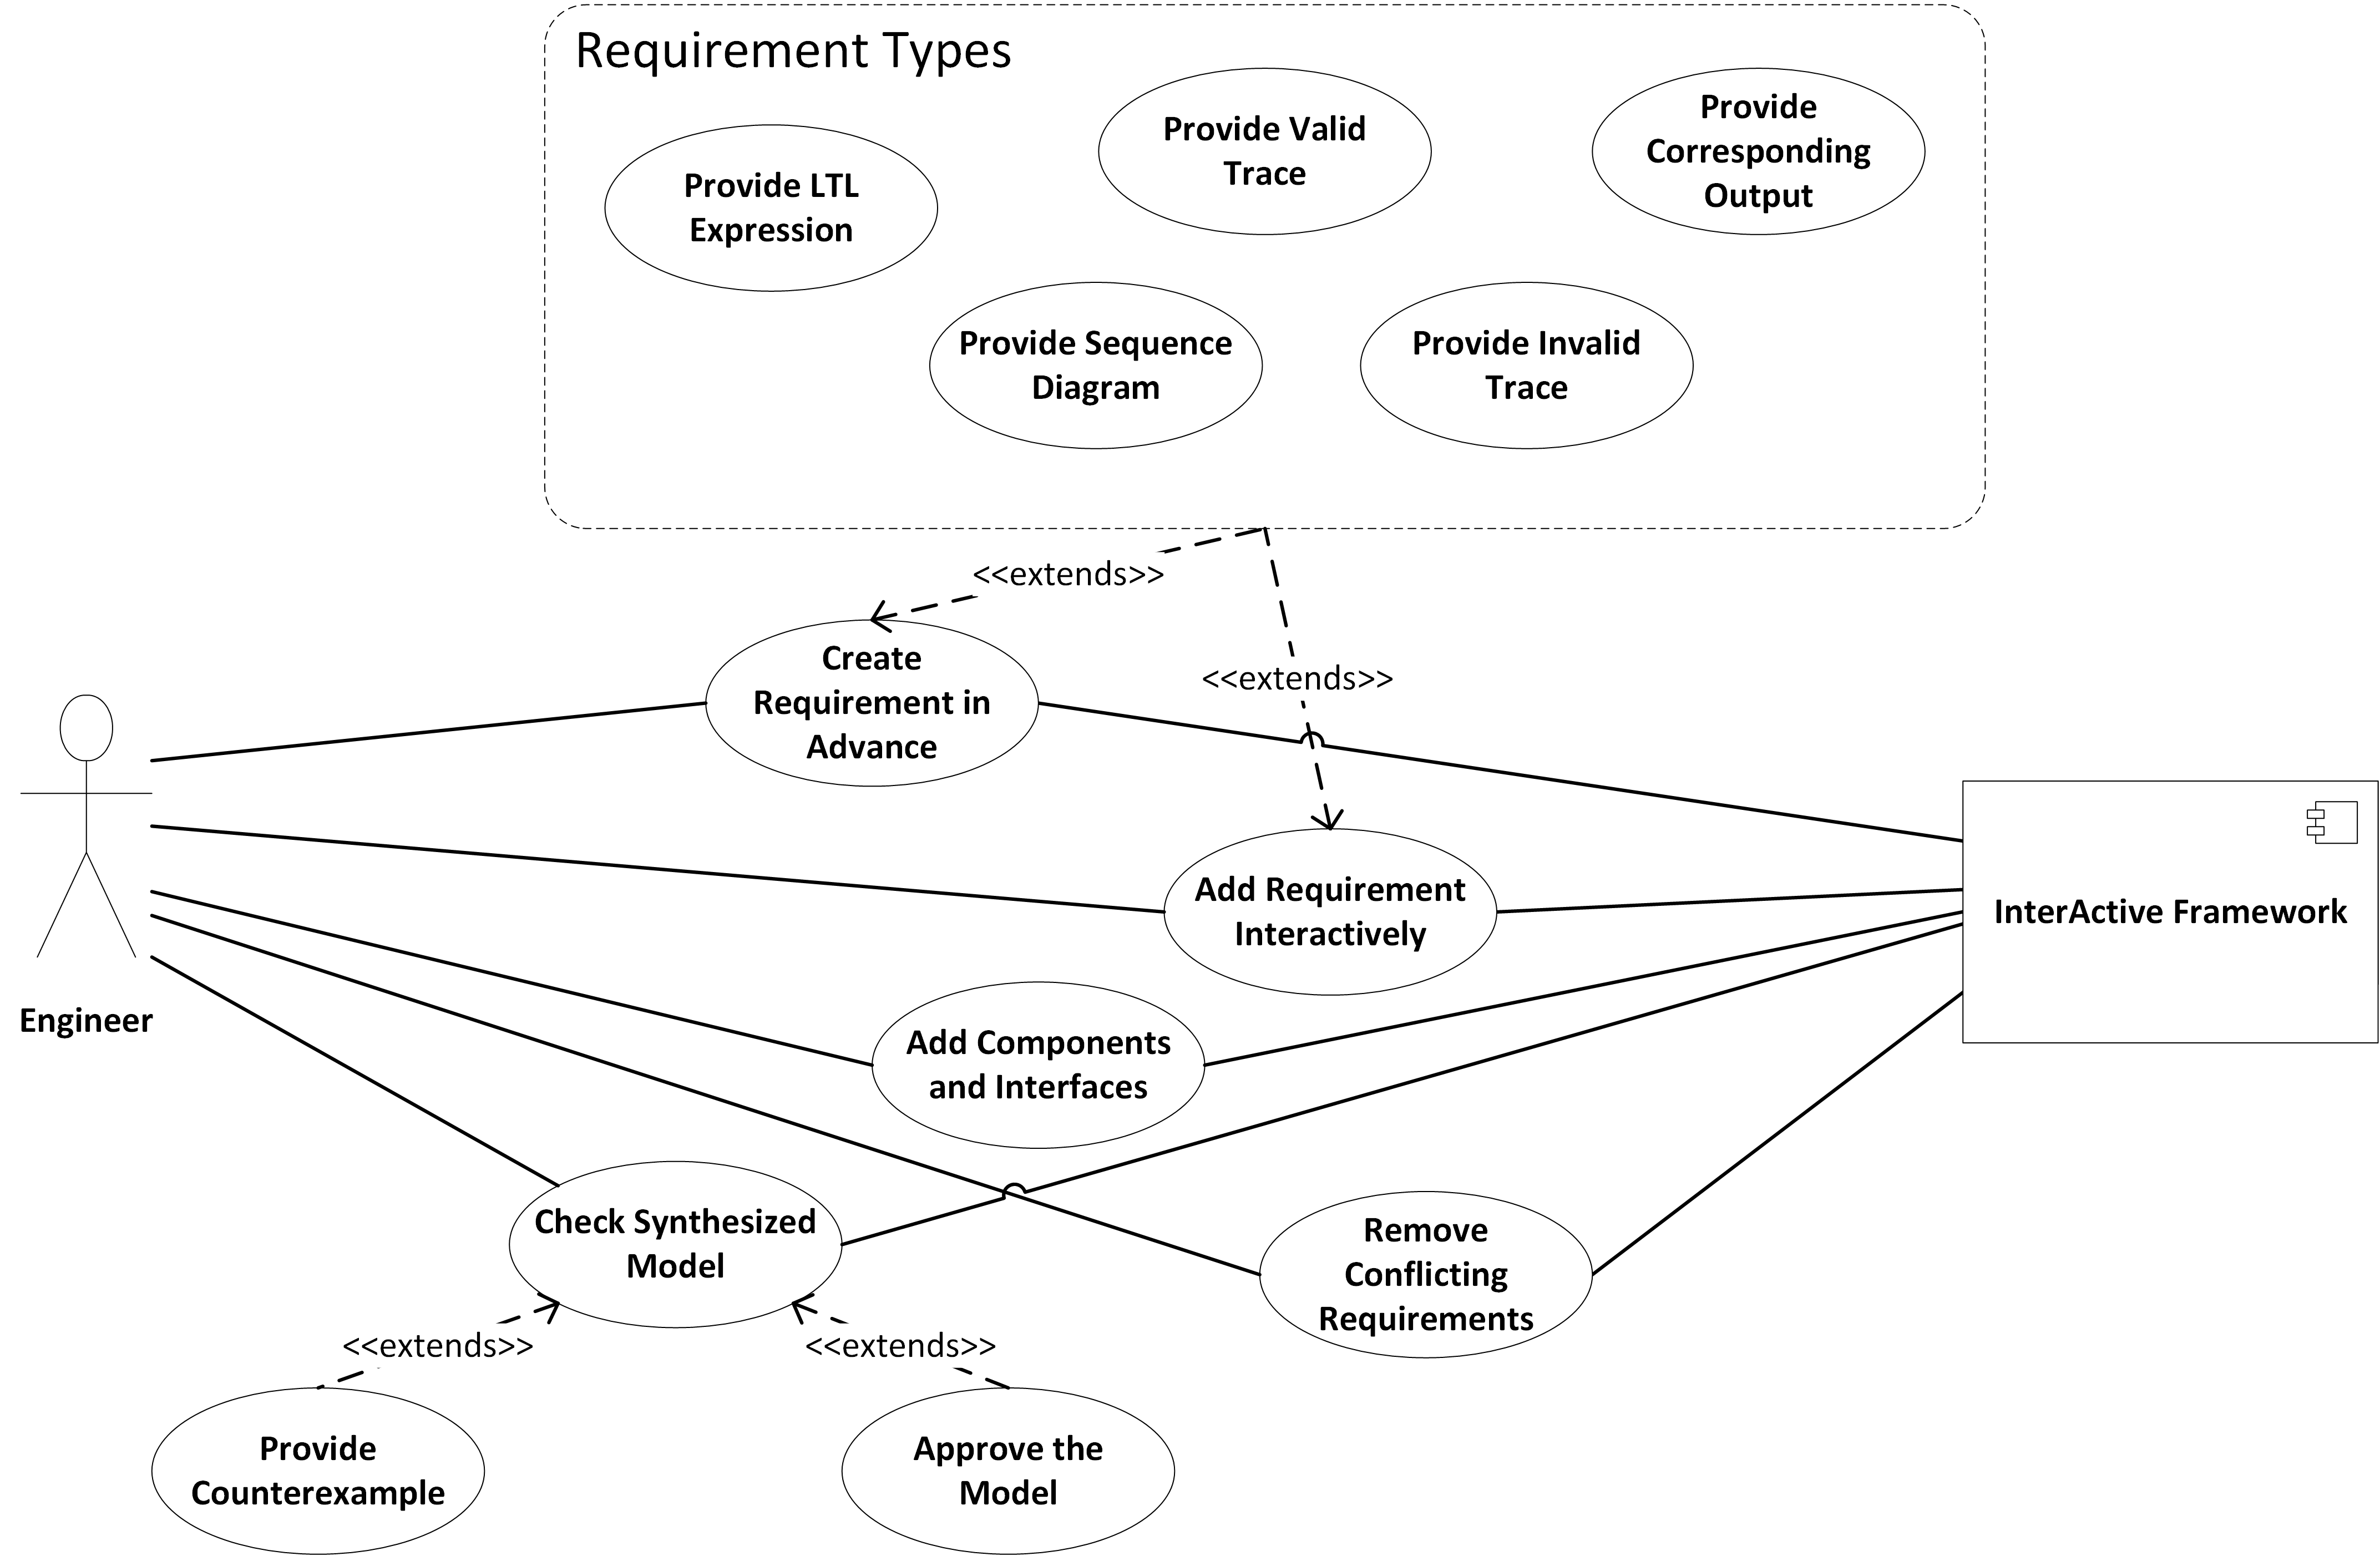
\includegraphics[width=150mm, keepaspectratio]{figures/methodology_interactiontypes.png}
	}
	\caption{Interaction types between the engineer and the ILE}
	\label{fig_methodology_interactiontypes}
\end{figure}

Our methodology is heavily based on the interaction of the user with the ILE. The different types of interacitons are summarized on Figure \ref{fig_methodology_interactiontypes} and are elaborated on in Subsection \ref{subs_reqtypes}. These interactions take place in a predefined order - the \textit{proposed workflow}, illustrated on Figure \ref{fig_methodology_workflow}. This workflow consists of two phases: first, an \textit{offline} one, and then an \textit{online} one, and ends with the serialization of the models. During the offline phase, the ILE offers little assistance, the designing engineer must determine the required details by other means. The interactive system design happens during the online phase. 

The individual steps in both the offline and the online phases have a predefined syntax with the corresponding, precisely defined semantics. Their common feature is the declarative way of describing the system components, which allows the engineer to focus solely on the expected behavior and acquire a minimal model exhibiting the specified functionality. The following subsections explain these steps in detail.

\begin{figure}[!ht] 
	\centering
	\fbox{
		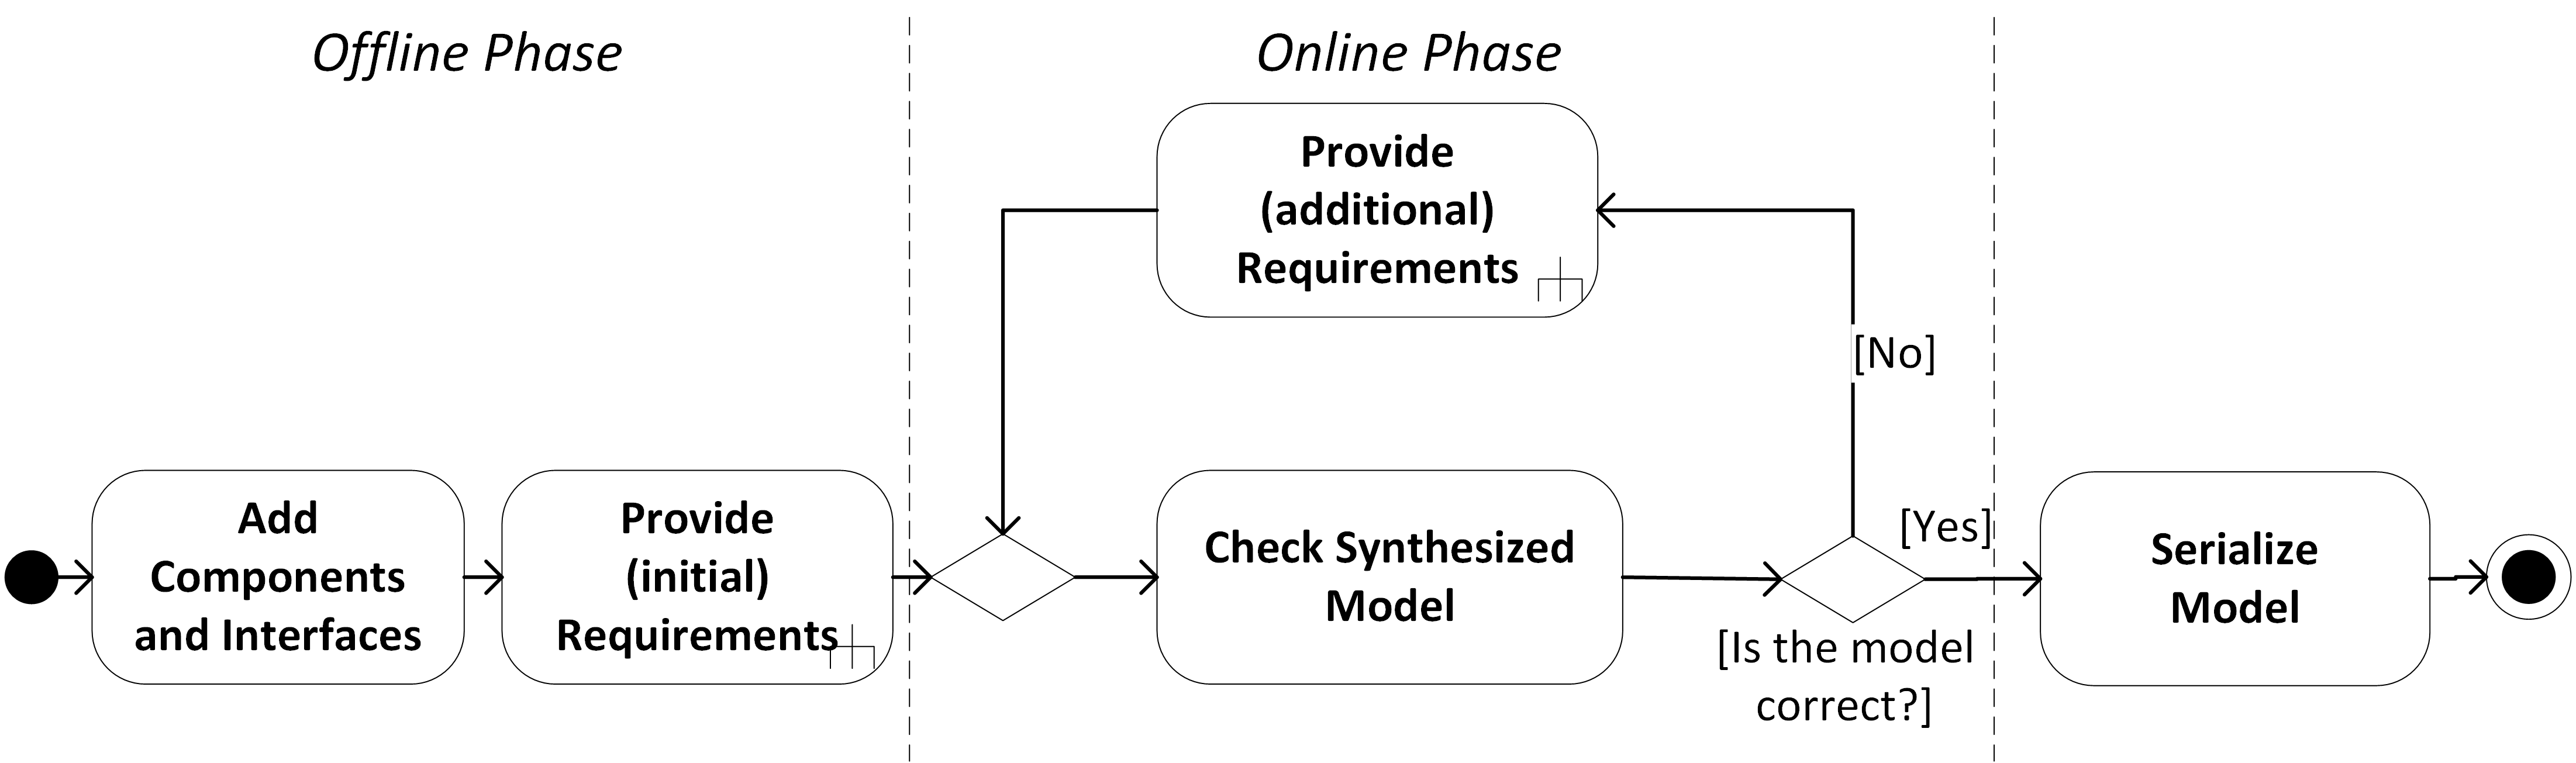
\includegraphics[width=150mm, keepaspectratio]{figures/methodology_workflow.png}
	}
	\caption{The Proposed Workflow}
	\label{fig_methodology_workflow}
\end{figure}
%TODO fork a komponenseknek

%---------------------------------------------------------------
\subsection{Component and Interface Definition} \label{subs_compdef}
%---------------------------------------------------------------
The first step of the workflow is the declaration of the system components. This happens in the offline phase, as the determination of the system components, their exact boundaries and interfaces is out of the scope of this work. Nonetheless, he engineer must provide the names of the system components, along with their interfaces - in other words their input- and output alphabets - before the workflow can proceed to the next step.

Users are encouraged to specify input and output characters qualified with interface names in the format 'Port.character', as this supplies the subsequent steps with essential information about the connections of the individual system components. For the sake of simplicity, this format is not necessarily used in the following examples.

The components are handled as independent systems in every other aspect. This results - among others - in the arbitrary ordering of the online behavior-learning phases, and the behavioral faults being limited to their components of origin (although this does not limit the propagation of errors through messages resulting from incorrect behavior).
The syntax of component and interface declarations is quite simple, as illustrated in Listing \ref{lst_compdef}.

\bigskip
\begin{lstlisting} [language=tex,caption=Example of a component declaration along with its interfaces,label=lst_compdef]
Components:
>component1 component2 component3
Input alphabet of component1:
>Input1.toggle Input2.interrupt
Output alphabet of component1: 
>Output1.red Output1.green Output1.blue
...
\end{lstlisting}

%---------------------------------------------------------------
\subsection{Requirement Types} \label{subs_reqtypes}
%---------------------------------------------------------------
During the workflow, the engineers can provide requirements in both the online and the offline phases. 

\begin{figure}[!ht] 
	\centering
	\fbox{
		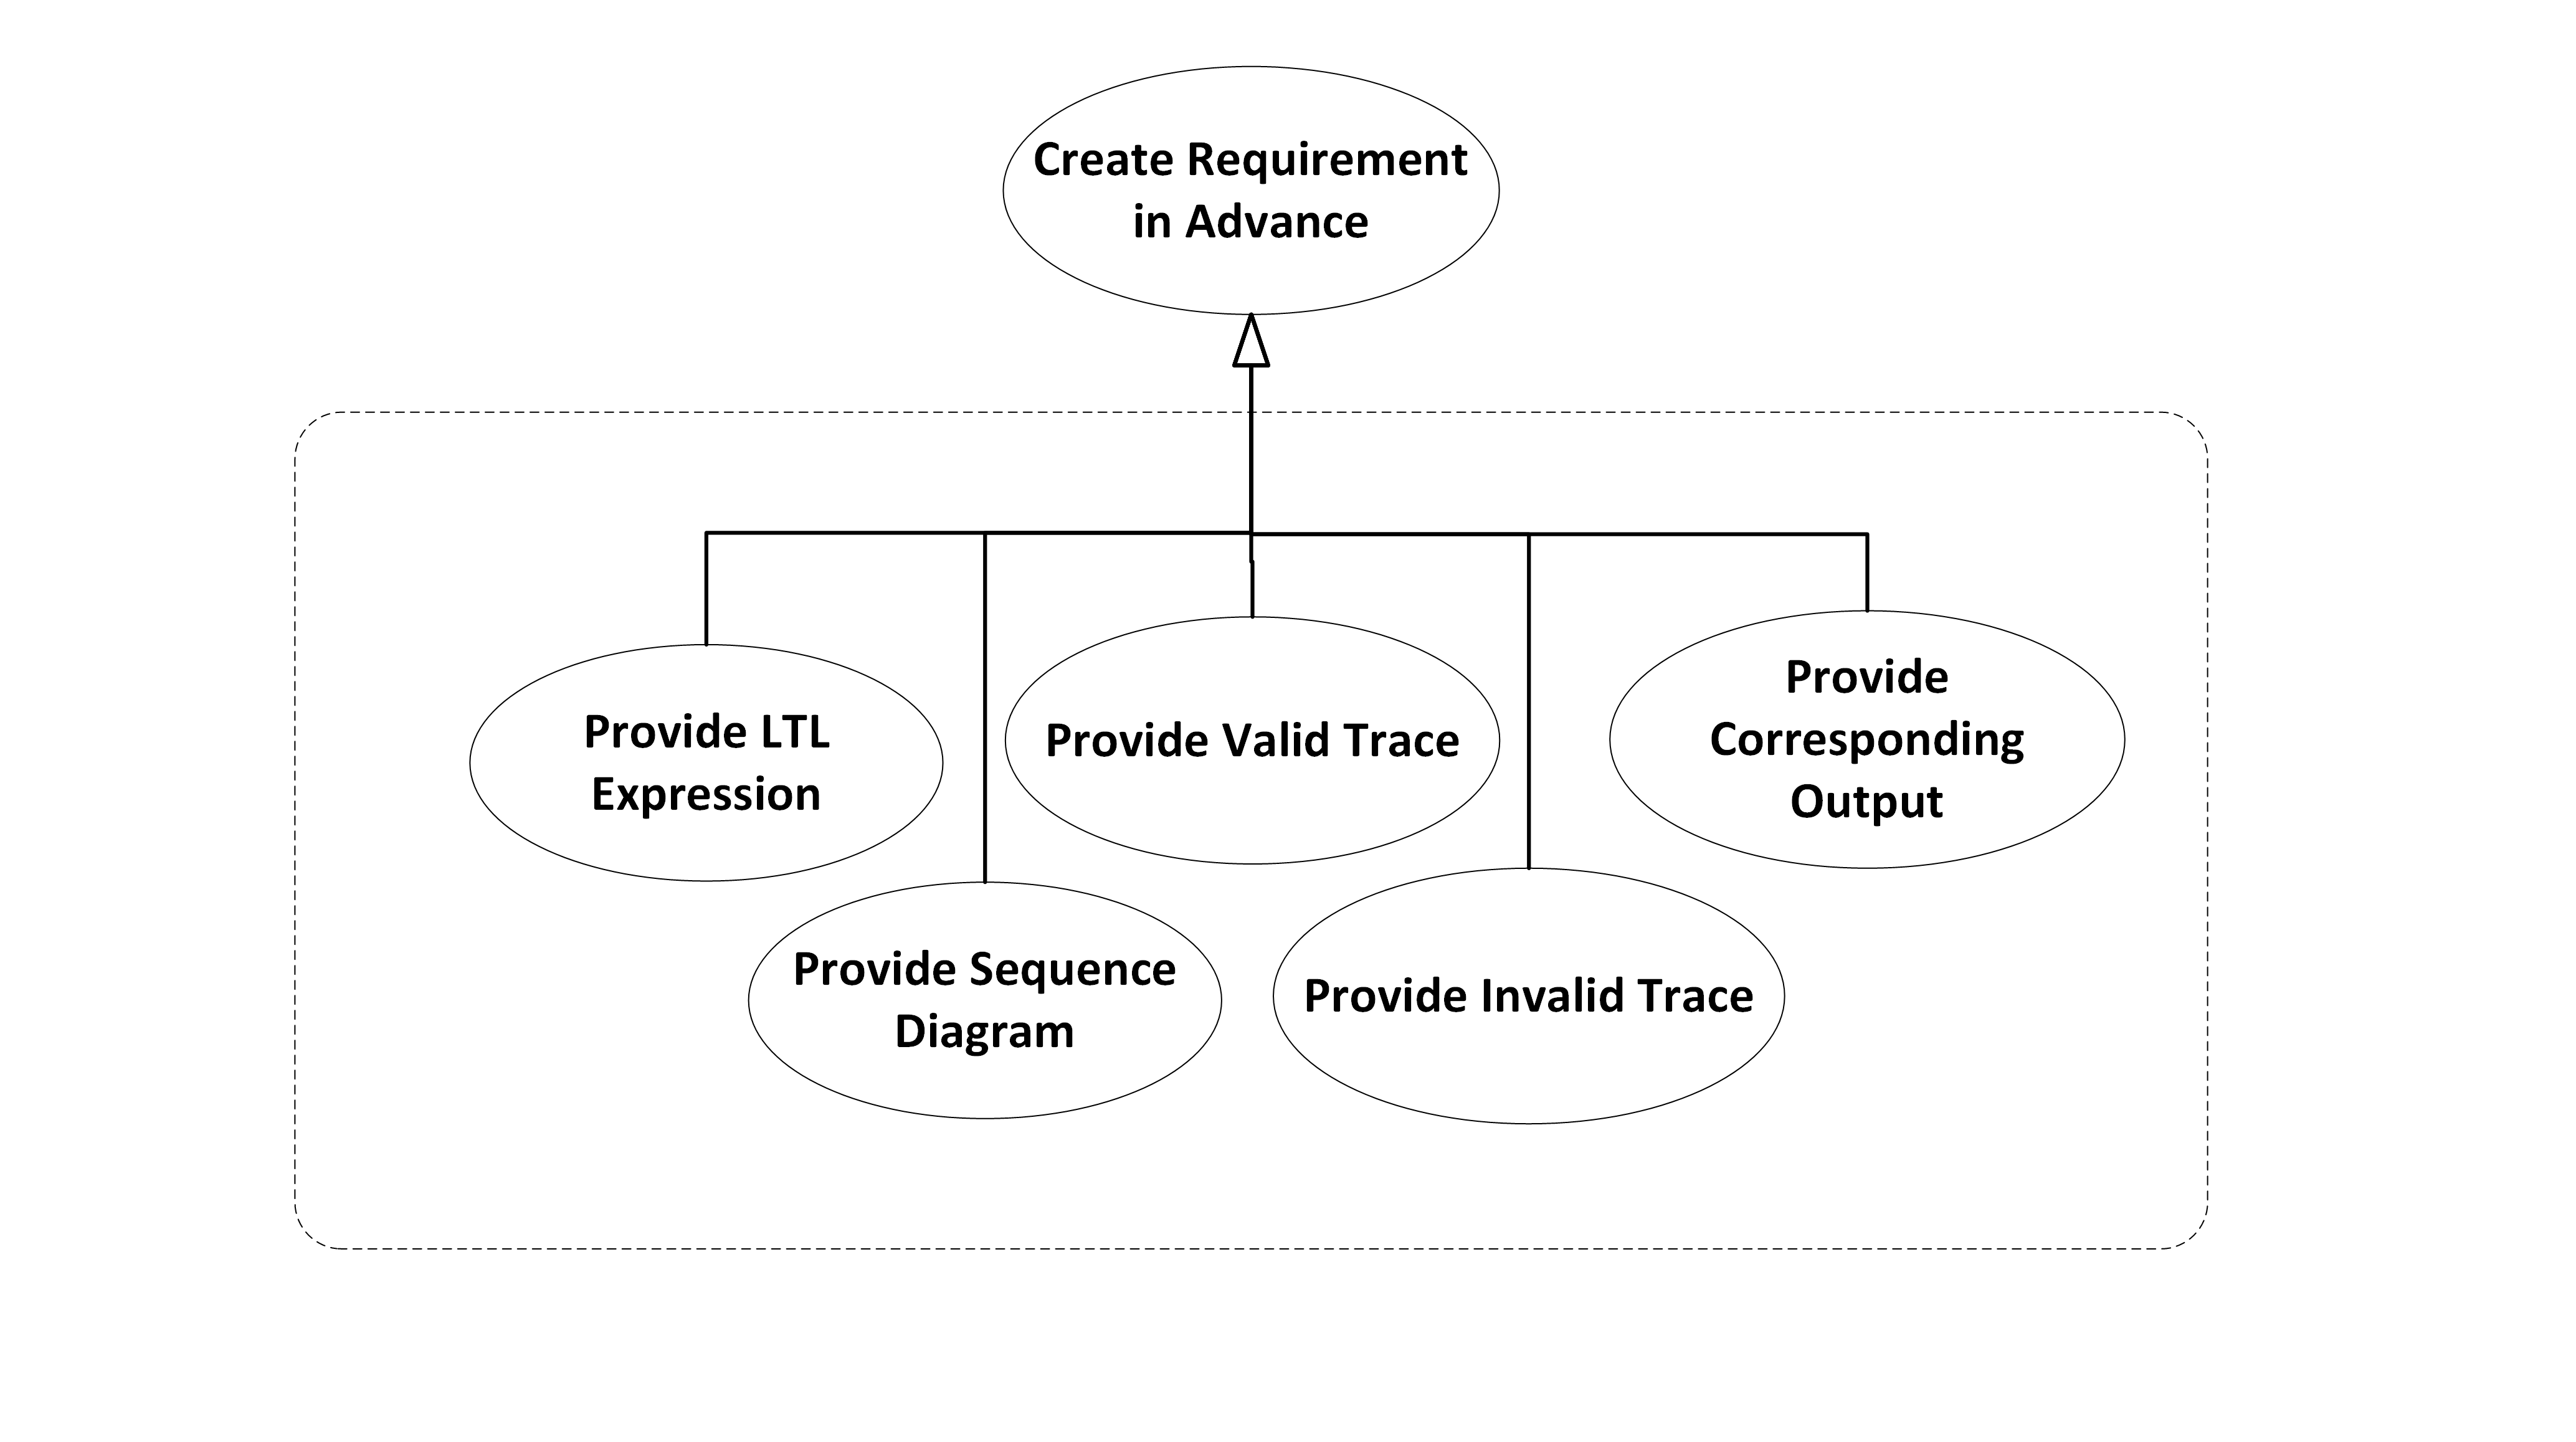
\includegraphics[width=150mm, keepaspectratio]{figures/methodology_requirementtypes.png}
	}
	\caption{The supported requirement types}
	\label{fig_requirementtypes}
\end{figure}

In the offline phase, this means that they add requirements they have formulated in advance. This is useful for more general requirements, with the scope of the whole component, conveniently formulated by program logic expressions, or long and complex traces.

In the online phase, adding requirements means answering the questions formulated by the algorithm about a yet unspecified behavior at a specific place in the trace currently being examined. This too can be answered through program logic - e.g. when the engineer realizes a general property during the model construction - but also through traces and through giving the corresponding output directly.

\textbf{Corresponding Output}
% TODO ref background: trace(-based)

This is the simplest way of specifying the behavior of the system, also containing the least amount of information among the different model types. To put simply, this means giving the output for a given input sequence, without any additional information. This supposedly answers the question of the ILE at \textit{one} given point, and that is the end of its scope.

Examples of corresponding output specification can be seen in Listing \ref{lst_iopair}.

\bigskip
\begin{lstlisting} [language=tex,caption=Examples of corresponding output specification,label=lst_iopair]
Offline: 
>input1 input2 input3 output

Online: 
>Output for [input1 input2 input3]:
>output3

(assuming input1/2/3 are from the input alphabet and output3 is from the output alphabet)
\end{lstlisting}

\textbf{Valid Trace}

Valid traces are a more complex form of specifying the corresponding output: it gives the corresponding output for any prefix of the contained input sequence. This might be useful, as usually the whole output sequence is taken into consideration when determining the output for some inputs. Thus, the ILE can obtain \textit{multiple} answers concerning the behaviors in question.

An example can be seen in Listing \ref{lst_validtrace}.

\bigskip
\begin{lstlisting} [language=tex,caption=Example of a valid trace,label=lst_validtrace]
Both offline and online:
>input1/output1 input2/output2 input3/output3

(assuming input1/2/3 are from the input alphabet and output1/2/3 are from the output alphabet) 
\end{lstlisting}

\textbf{Sequence Diagram}
%TODO ref backgr UML

UML-like sequence diagrams - the ones introduced in [TODO ref backgr] - are an even more complex form of trace-based models, as they can contain several traces, due to them having various combined fragments for branching the behavior - like \textit{alt} and \textit{opt} - and for referencing behaviors specified elsewhere - like \textit{ref}.

Sequence diagrams can also be used to model infinite behavior, which results in containing plenty of information, which in turn results in possibly answering \textit{several} questions formulated by the ILE.

%TODO
An example for the application of sequence diagrams can be seen on [TODO insert example]

It is important to note, that the specification and integration of sequence diagrams into this framework is not yet complete. 

\textbf{Trace to Exclude}

Invalid traces are similar to valid traces, with the difference that the contained behavior must not appear in the resulting model. They are most useful for small output alphabets, or when the range of possible behaviors is otherwise contained - e.g. through program logic expressions or several other excluded traces.

They can also be used to formulate requirements when the determination of the correct behavior does not directly follow from them: when specifying the behavior in question, the ILE will signal any conflicting requirements for the examined input sequences and require the user to remove one - thus facilitating the enforcement of these requirements too.

An example for invalid traces can be seen in Listing \ref{lst_invalidtrace}.

\bigskip
\begin{lstlisting} [language=tex,caption=Example of a trace to exclude,label=lst_invalidtrace]
Both offline and online:
>input4/output4 input5/output5

(assuming input4/5 are from the input alphabet and output4/5 are from the output alphabet) 
\end{lstlisting}

\textbf{LTL Expression}
%TODO ref backgr LTL
%TODO ref backgr LTS

LTL expressions are a highly complex type of program logic-based requirement specification: they can be used to formulate propositional logic expressions with temporal connectives over \textit{paths} of a \textit{base model}, as described in [TODO ref backgr]. 

For our application, we introduce our own LTL expression language with its own syntax and semantics - although attempting to keep it similar to other generally known variants, especially that of SPOT [TODO cite]. The full syntax of the LTL expressions - also determining the operator precedence - can be seen in Listing \ref{lst_ltlfullsyntax}.

The base model of the LTL expressions is the LTS [TODO ref backgr] interpretation of the component under learning. This means, that the set of atomic propositions that can be used in these expressions are the possible labels of the transitions, which are the elements of the input and the output alphabets of the component. The model synthesis takes place assuming event semantics - exactly one input and one output event happening at any given time. For this reason, we also introduced these semantics to the LTL expressions: the conjunction of exactly one input and one output character must hold at any given point in time for it to be considered correct - and every other character must be negated at the same point. This also entails, that given another character not explicitly negated at that point, it is assumed to be automatically negated, and in the case that no proposition is declared explicitly to hold, it is assumed that either one of the non-explicitly negated characters hold. 

The semantics of the supported temporal connectives, and other aspects of the LTL semantics in general, are similar to those described in [TODO ref backgr] %TODO

Examples for a valid LTL expressions can be seen in Listing \ref{lst_ltlex}.

\bigskip
\begin{lstlisting} [language=tex,caption=Examples of LTL expressions,label=lst_ltlex]
Assuming Control.interrupt and toggle are from the input alphabet and blinkingYellow is from the output alphabet, both offline and online:
>F(interrupt -> X(G(toggle) -> G(blinkingYellow)))

Assuming the output alphabet also contains red, yellow and green, it is equivalent to:
>F(interrupt&!toggle -> X(G(toggle&!interrupt) -> G(blinkingYellow&!red&!yellow&!green)))
\end{lstlisting}

It is important to note, that the specification of our LTL variant is not yet complete: for the compactness of requirement specifications it would make sense to integrate additional well-known boolean operators - like XOR (exclusive-or) - and temportal connectives - such as WB (weak-before) and R (release) - into the language. 

%---------------------------------------------------------------
\subsection{Conflicting Requirements} \label{subs_conf}
%---------------------------------------------------------------
The requirements the designing engineer provides the ILE with may easily be conflicting, especially in case of LTL expressions and invalid traces - that describe possibly infinite sets of behaviors. For this reason, it is essential for the system to provide some kind of conflict handling within the practical boundaries of the available resources. 

This problem is a difficult and resource intensive task for algorithmic reasons elaborated later. Consequently, the ILE only guarantees to handle the conflict, when it also interferes with the model synthesis, in which case, the user is asked to remove one of the conflicting models, before the analysis of the behavior can proceed.

\begin{figure}[!ht] 
	\centering
	%\fbox{
		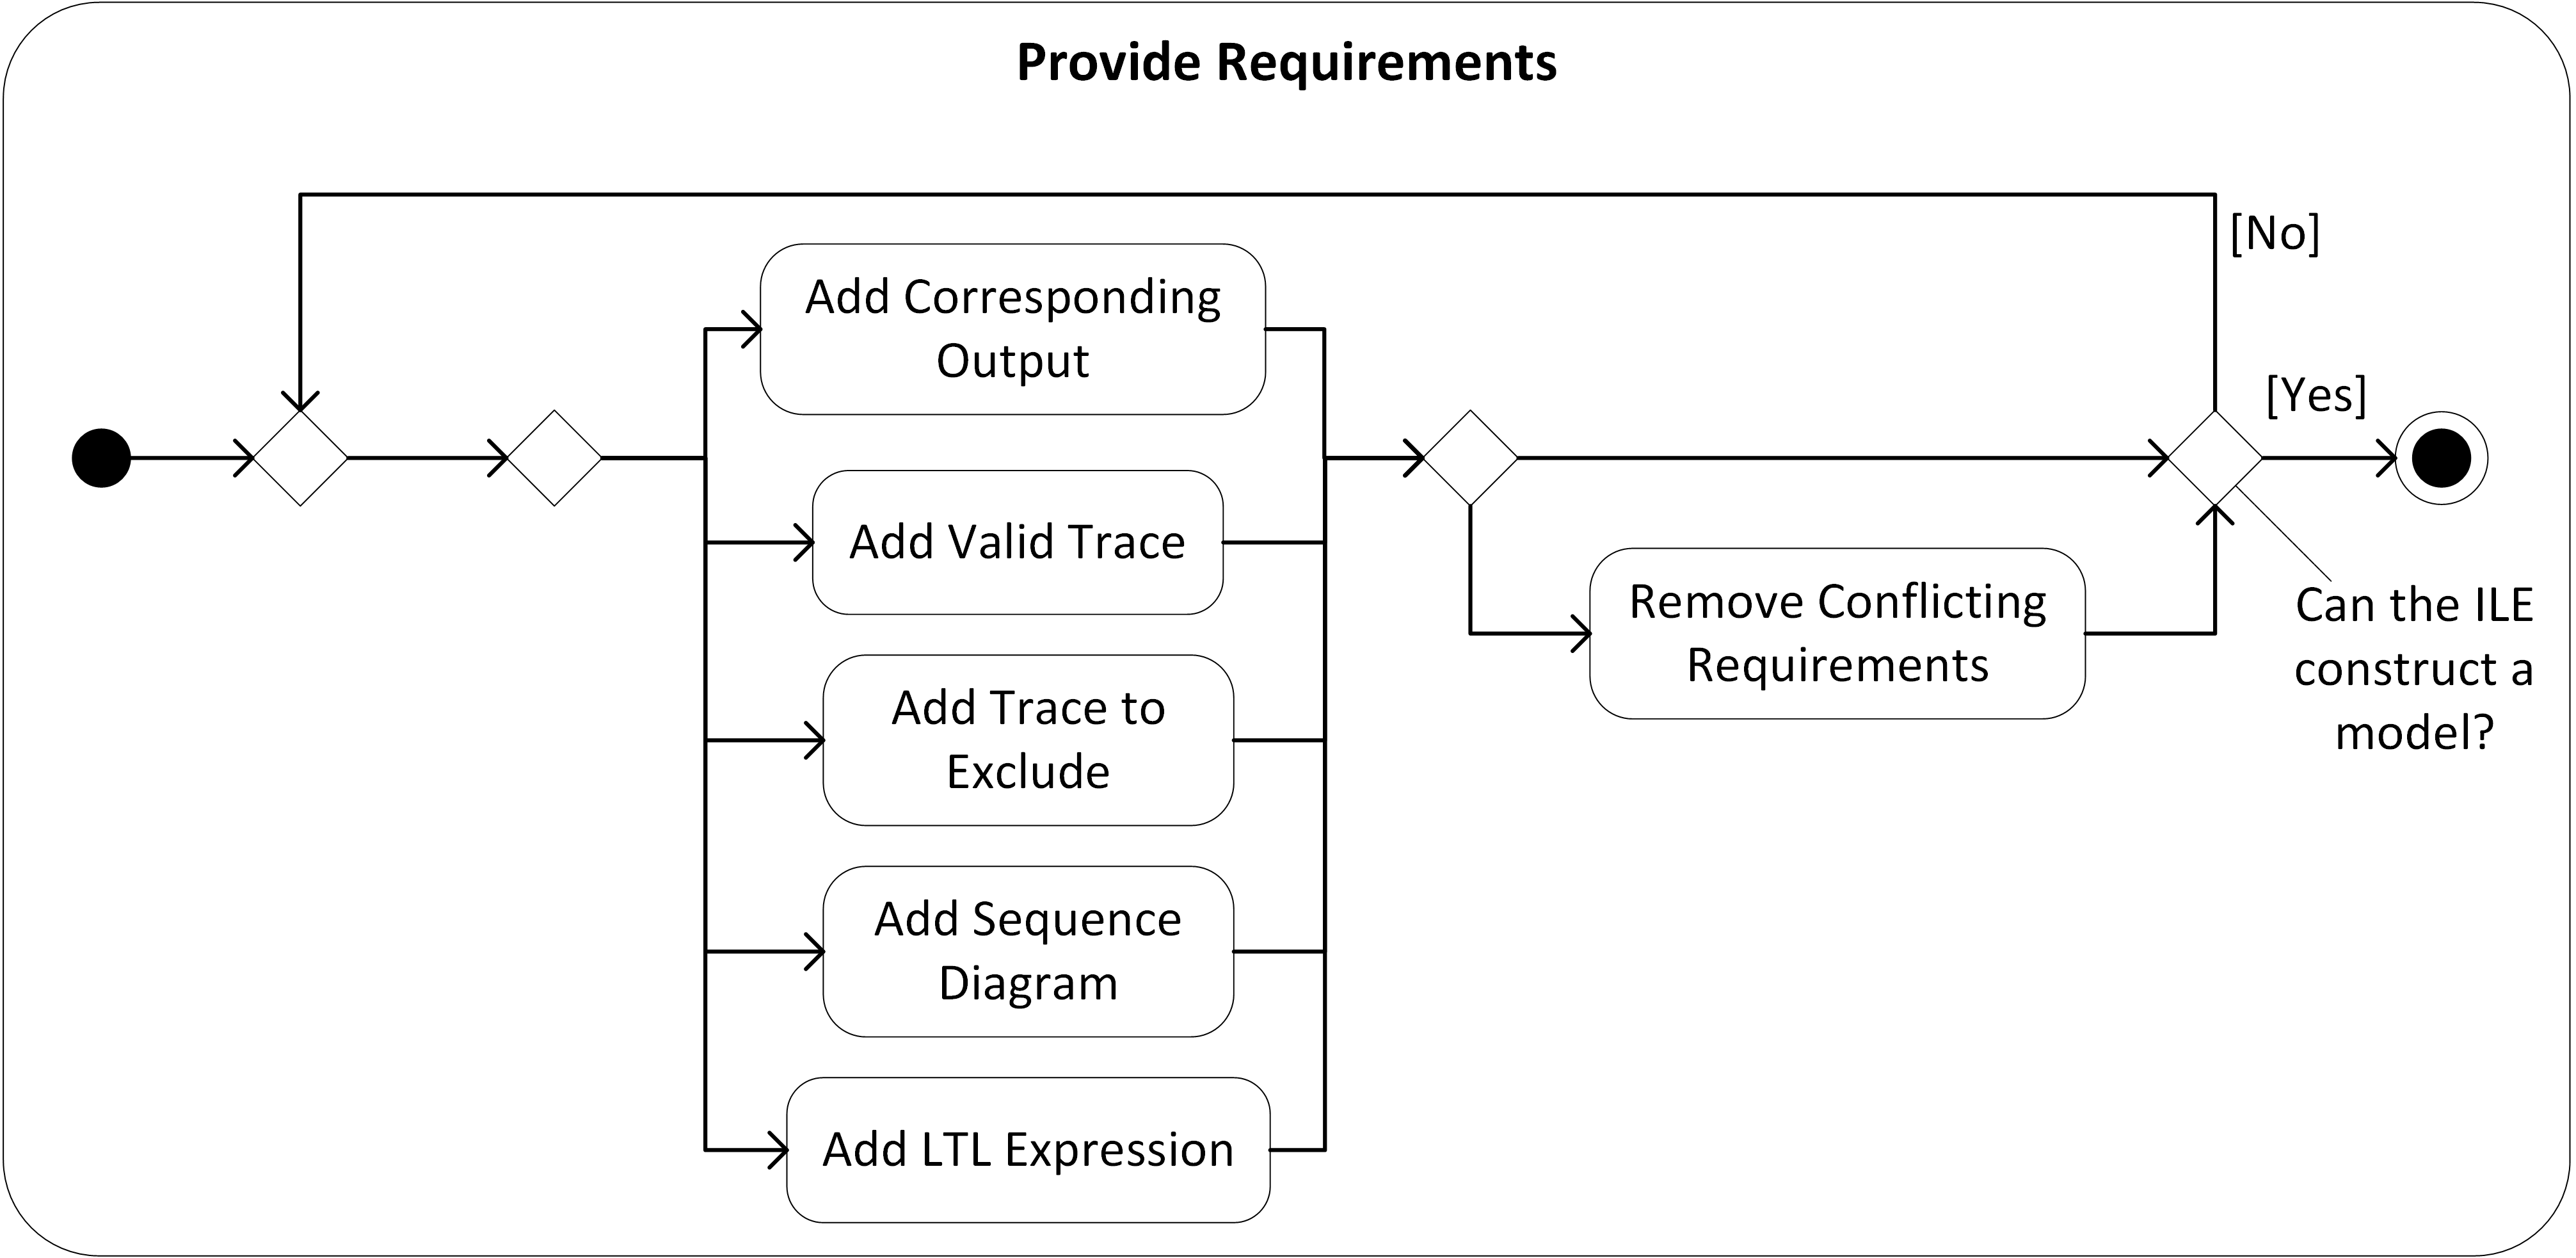
\includegraphics[width=130mm, keepaspectratio]{figures/methodology_providerequirementsworkflow.png}
	%}
	\caption{The process of adding a requirement}
	\label{fig_providerequirementsworkflow}
\end{figure}


As conflicts only become apparent during the online phase of the workflow, the conflict handling is only present there. However, conflicts that were introduced earlier are also discovered and resolved in that phase. An example of a requirement conflict handling can be seen in Listing \ref{lst_conflicthandling}.

\bigskip
\begin{minipage}{\linewidth}
\begin{lstlisting} [language=tex,caption=Example of a requirement conflict handling,label=lst_conflicthandling]
	TODO EXAMPLE
	TODO EXAMPLE
\end{lstlisting}%TODO
\end{minipage}

%---------------------------------------------------------------
\subsection{Checking the Correctness of the Synthesized Model} \label{subs_eq}
%---------------------------------------------------------------
During the online phase, whenever ILE assumes that it has gathered enough information to construct a model for the given component, the engineer if offered with a possible model representing the current state of the model synthesis - the equivalent of an equivalence query in automaton learning algorithms. This model can either be approved, or a counterexample is required from the user, where the model does not meet the - not yet specified - requirements.

The proposed equivalence model is a deterministic automaton, which, based on the information provided by the user, can be incomplete in multiple ways. The behavior of the proposed model can differ from the learned systems because of lacking information, in which case the user (acting as the equivalence oracle of the learning) needs to provide the separating behavior. Another reason for incompleteness is newly discovered states, the behavior of which is unknown based on their input signatures. This case prompts the user to evaluate the validity of state separation and is required to provide the lacking information. If, for some reason the hypothesized behavior is contradicting that of the imagined system (by the users oversight in providing requirements), the actual, conflicting requirement can be provided to guide the learning algorithm through the process described in Subsection \ref{subs_conf}.

If the model is accepted, the workflow can attempt to proceed to the next step - the serialization of the model. If a counterexample is provided, the online phase resumes and the system design continues until the next possible model is reached.

Examples of models offered in equivalence queries can be seen on Figure \ref{fig_methodology_eqex}.

\begin{figure}[!ht] 
	\centering
	\fbox{
		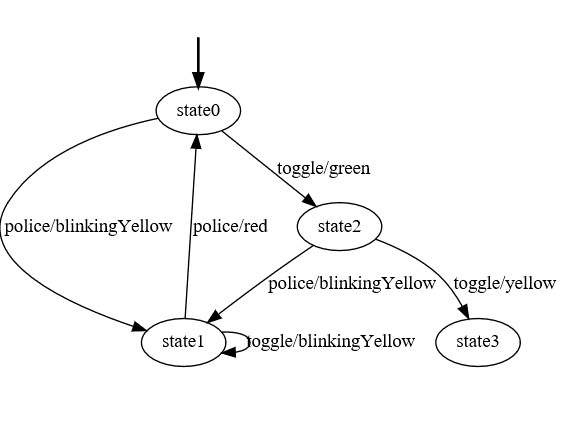
\includegraphics[height=50mm, keepaspectratio]{figures/methodology_eqex1.png}
	}
	\fbox{
		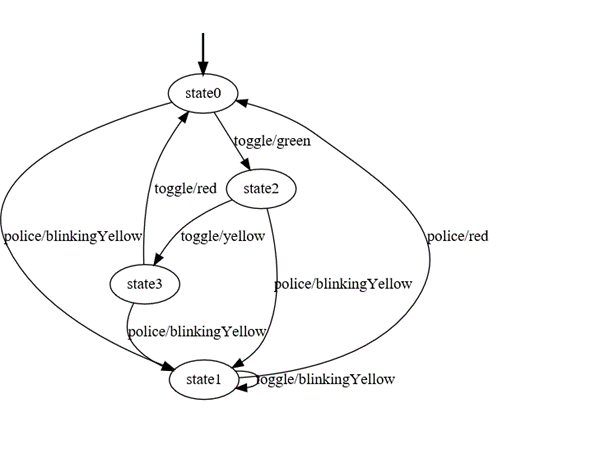
\includegraphics[height=50mm, keepaspectratio]{figures/methodology_eqex2.png}
	}
	\caption{Equivalence query for an incomplete model (\textit{left}) and the final model (\textit{right})}
	\label{fig_methodology_eqex}
\end{figure}

%---------------------------------------------------------------
\subsection{The Resulting System Model} \label{subs_resultingmodel}
%---------------------------------------------------------------
When each of the component models declared during the first step of the workflow are completed, the resulting system model can be serialized and handed over to the engineer for further extensions or to use it for any of its possible applications. This serialization can happen in various formalisms.

%TODO ref 
One such possible formalism is the serialization to a Gamma statechart, introduced in [TODO ref backgr]. Gamma statecharts are high-level state-based models, to which every functionality offered by the Gamma Statechart Composition Framework can be applied. Our framework offers full-scale Gamma serialization: when choosing this formalism, a whole project will be created, along with interface definitions, component definitions - for each of the previously declared components, with the synthesized behavior - and a composite system definition, connecting the components based on the names of their interfaces.

%TODO ref
Another possibility is the serialization to the Mealy machine formalism of the framework - as presented when checking the correctness of the model. This results in a lower-level set of independent models, with a completely different set of applications.

%TODO interface definitions vs component diagram
[TODO figure comes here: [comps\&interfaces | resulting structure]]
\clearpage
%----------------------------------------------------------------------------
\section{Overview of the Architecture} \label{sec_architecture}
%----------------------------------------------------------------------------

The architecture of the ILE consists of two main components: the automata learning algorithm - which is responsible for the model synthesis procedure, thus the course of the learning - and the interactive oracle - investigating the membership of the given input sequences in the languages of the models given by the user on one side and interacting with the user on the other. This architecture is depicted on Figure \ref{fig_architcture_ileoverview}. The following subsections elaborate on the connections and details of these components. 

\begin{figure}[!ht] 
	\centering
	\fbox{
		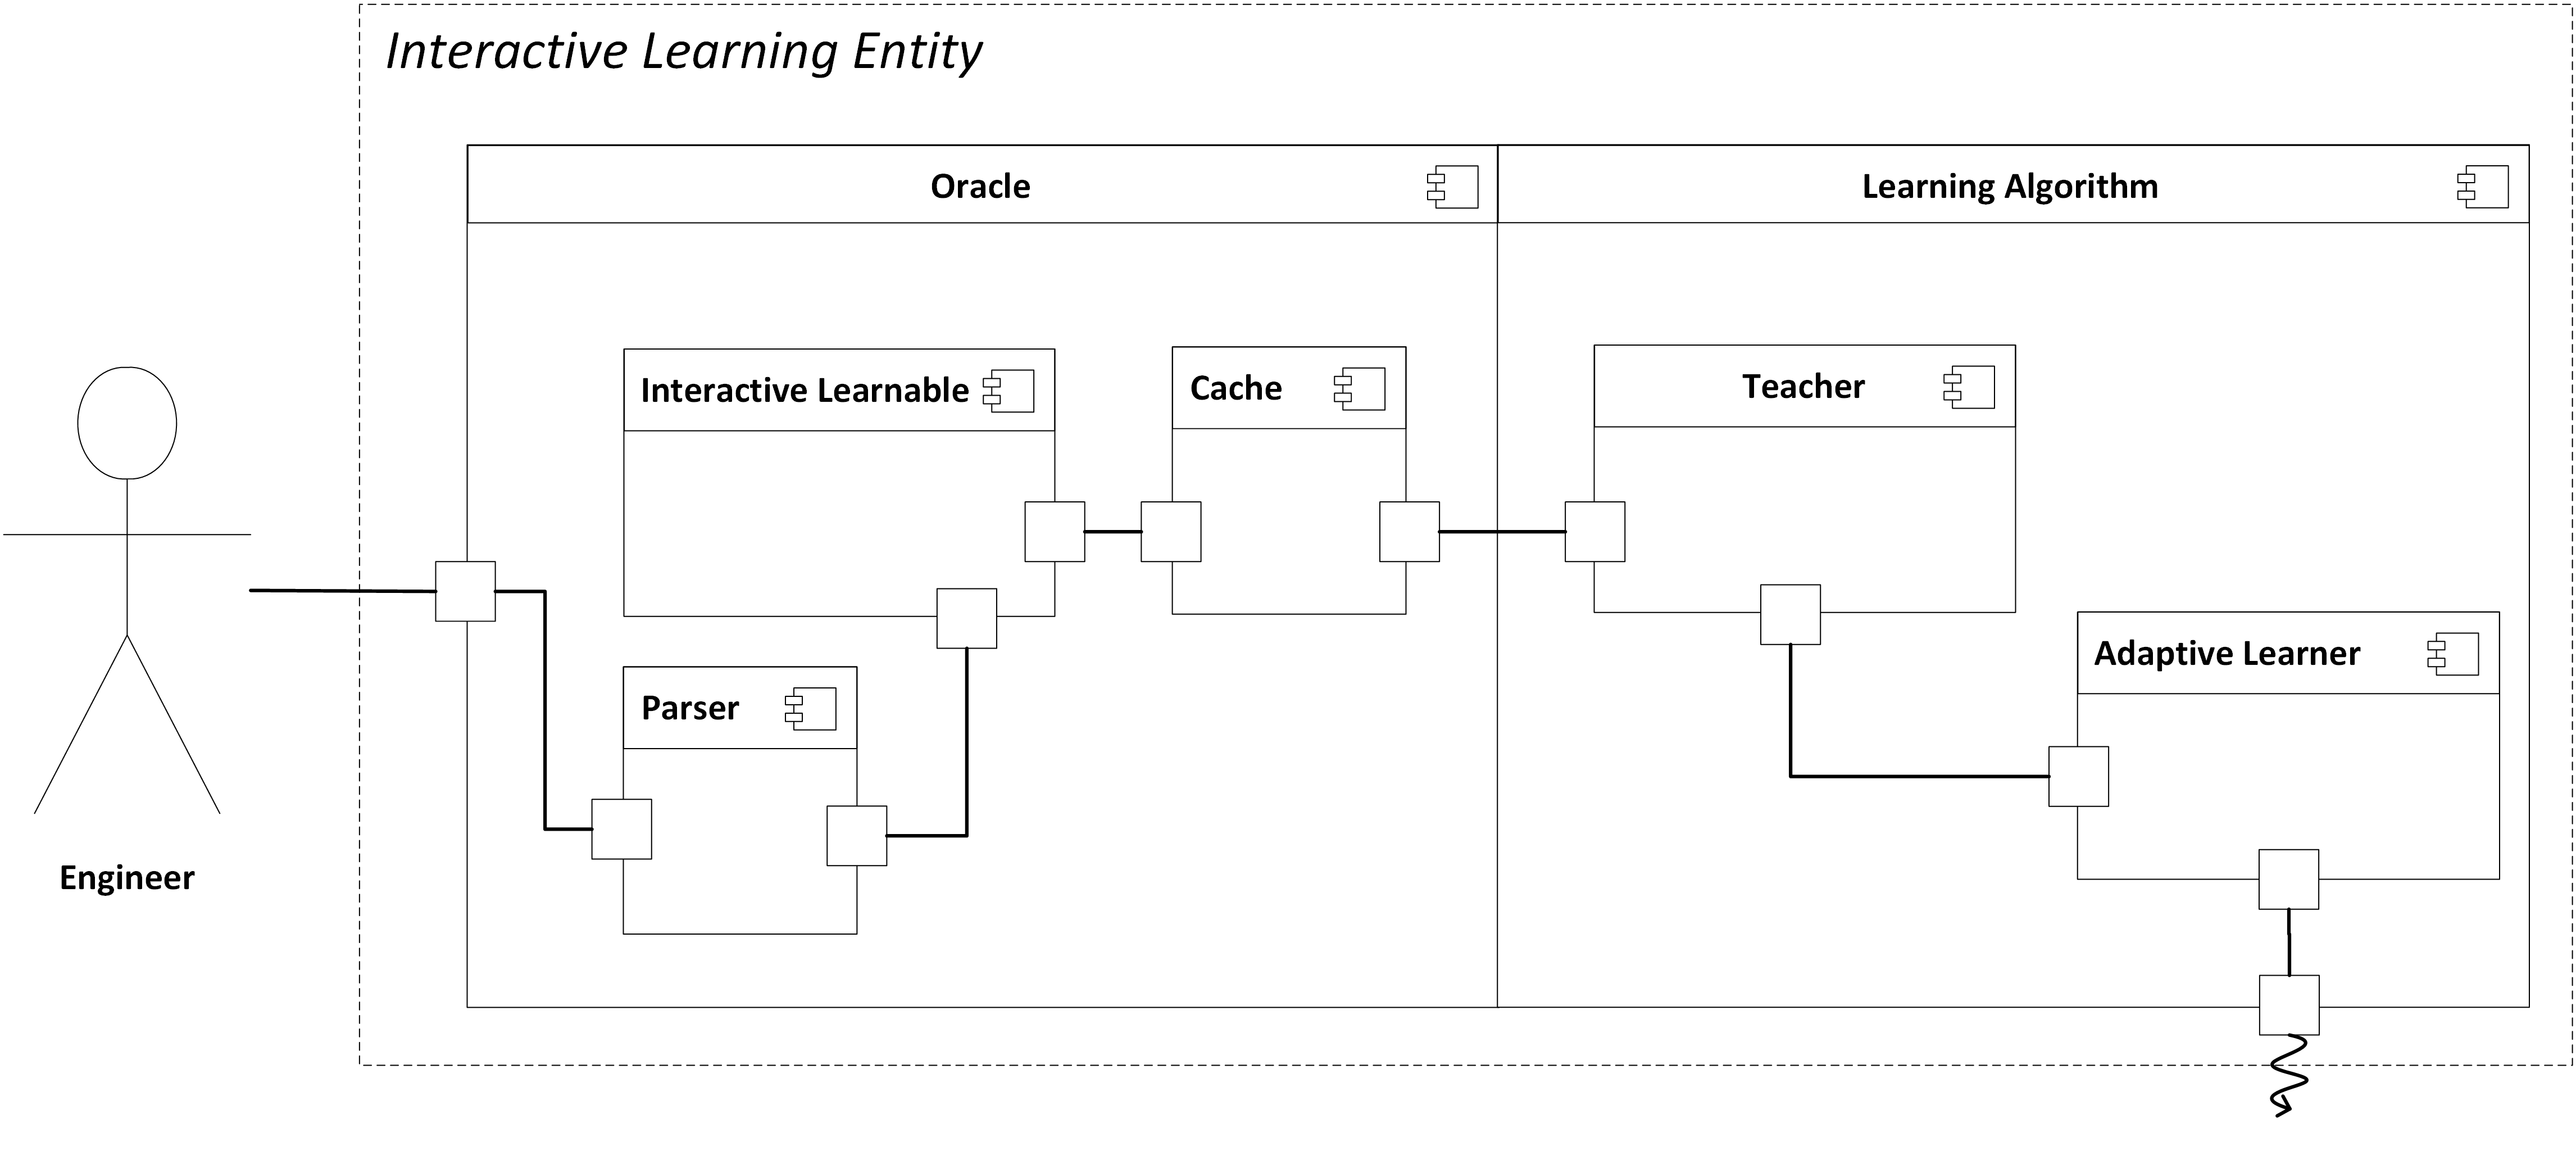
\includegraphics[width=150mm, keepaspectratio]{figures/architecture_ileoverview.png}
	}
	\caption{High-level architecture of the components of the ILE} 
	\label{fig_architcture_ileoverview}
\end{figure}

%---------------------------------------------------------------
\subsection{Automata Learning in the Framework} \label{subs_automatalearningintheframework}
%---------------------------------------------------------------
As discussed in [TODO: ref to background], active automaton learning algorithms work through a teacher and a learner component. While traditionally, the queries asked through the teacher are automated - by known or derived information and equivalence algorithms - in order to achieve an interactive algorithm a new approach was needed. Figure \ref{fig_architcture_ileoverview} shows an Adaptive Learner delegating its queries through the teacher  component to an interactive oracle, which delegates the relevant questions to the user. While the abstract approach presented in Figure \ref{fig_architcture_ileoverview} does enable interactive learning (by delegating every single query to the user), in practical use cases this proves to be infeasible simply because of the amount of queries needed to learn a model. In order to overcome this boundary, optimizations were made to automate a subset of queries, and a new active automaton learning approach was designed to heuristically control the design space.
%TODO (the teacher delegates the questions to the interactive learnable, which in turn delegates to the user ...)

%---------------------------------------------------------------
\subsection{Interactive Learnable} \label{subs_oracle}
%---------------------------------------------------------------
(hogyan foglalja össze a partial modeleket)
%TODO 
\begin{figure}[!ht] 
	\centering
	%\fbox{
	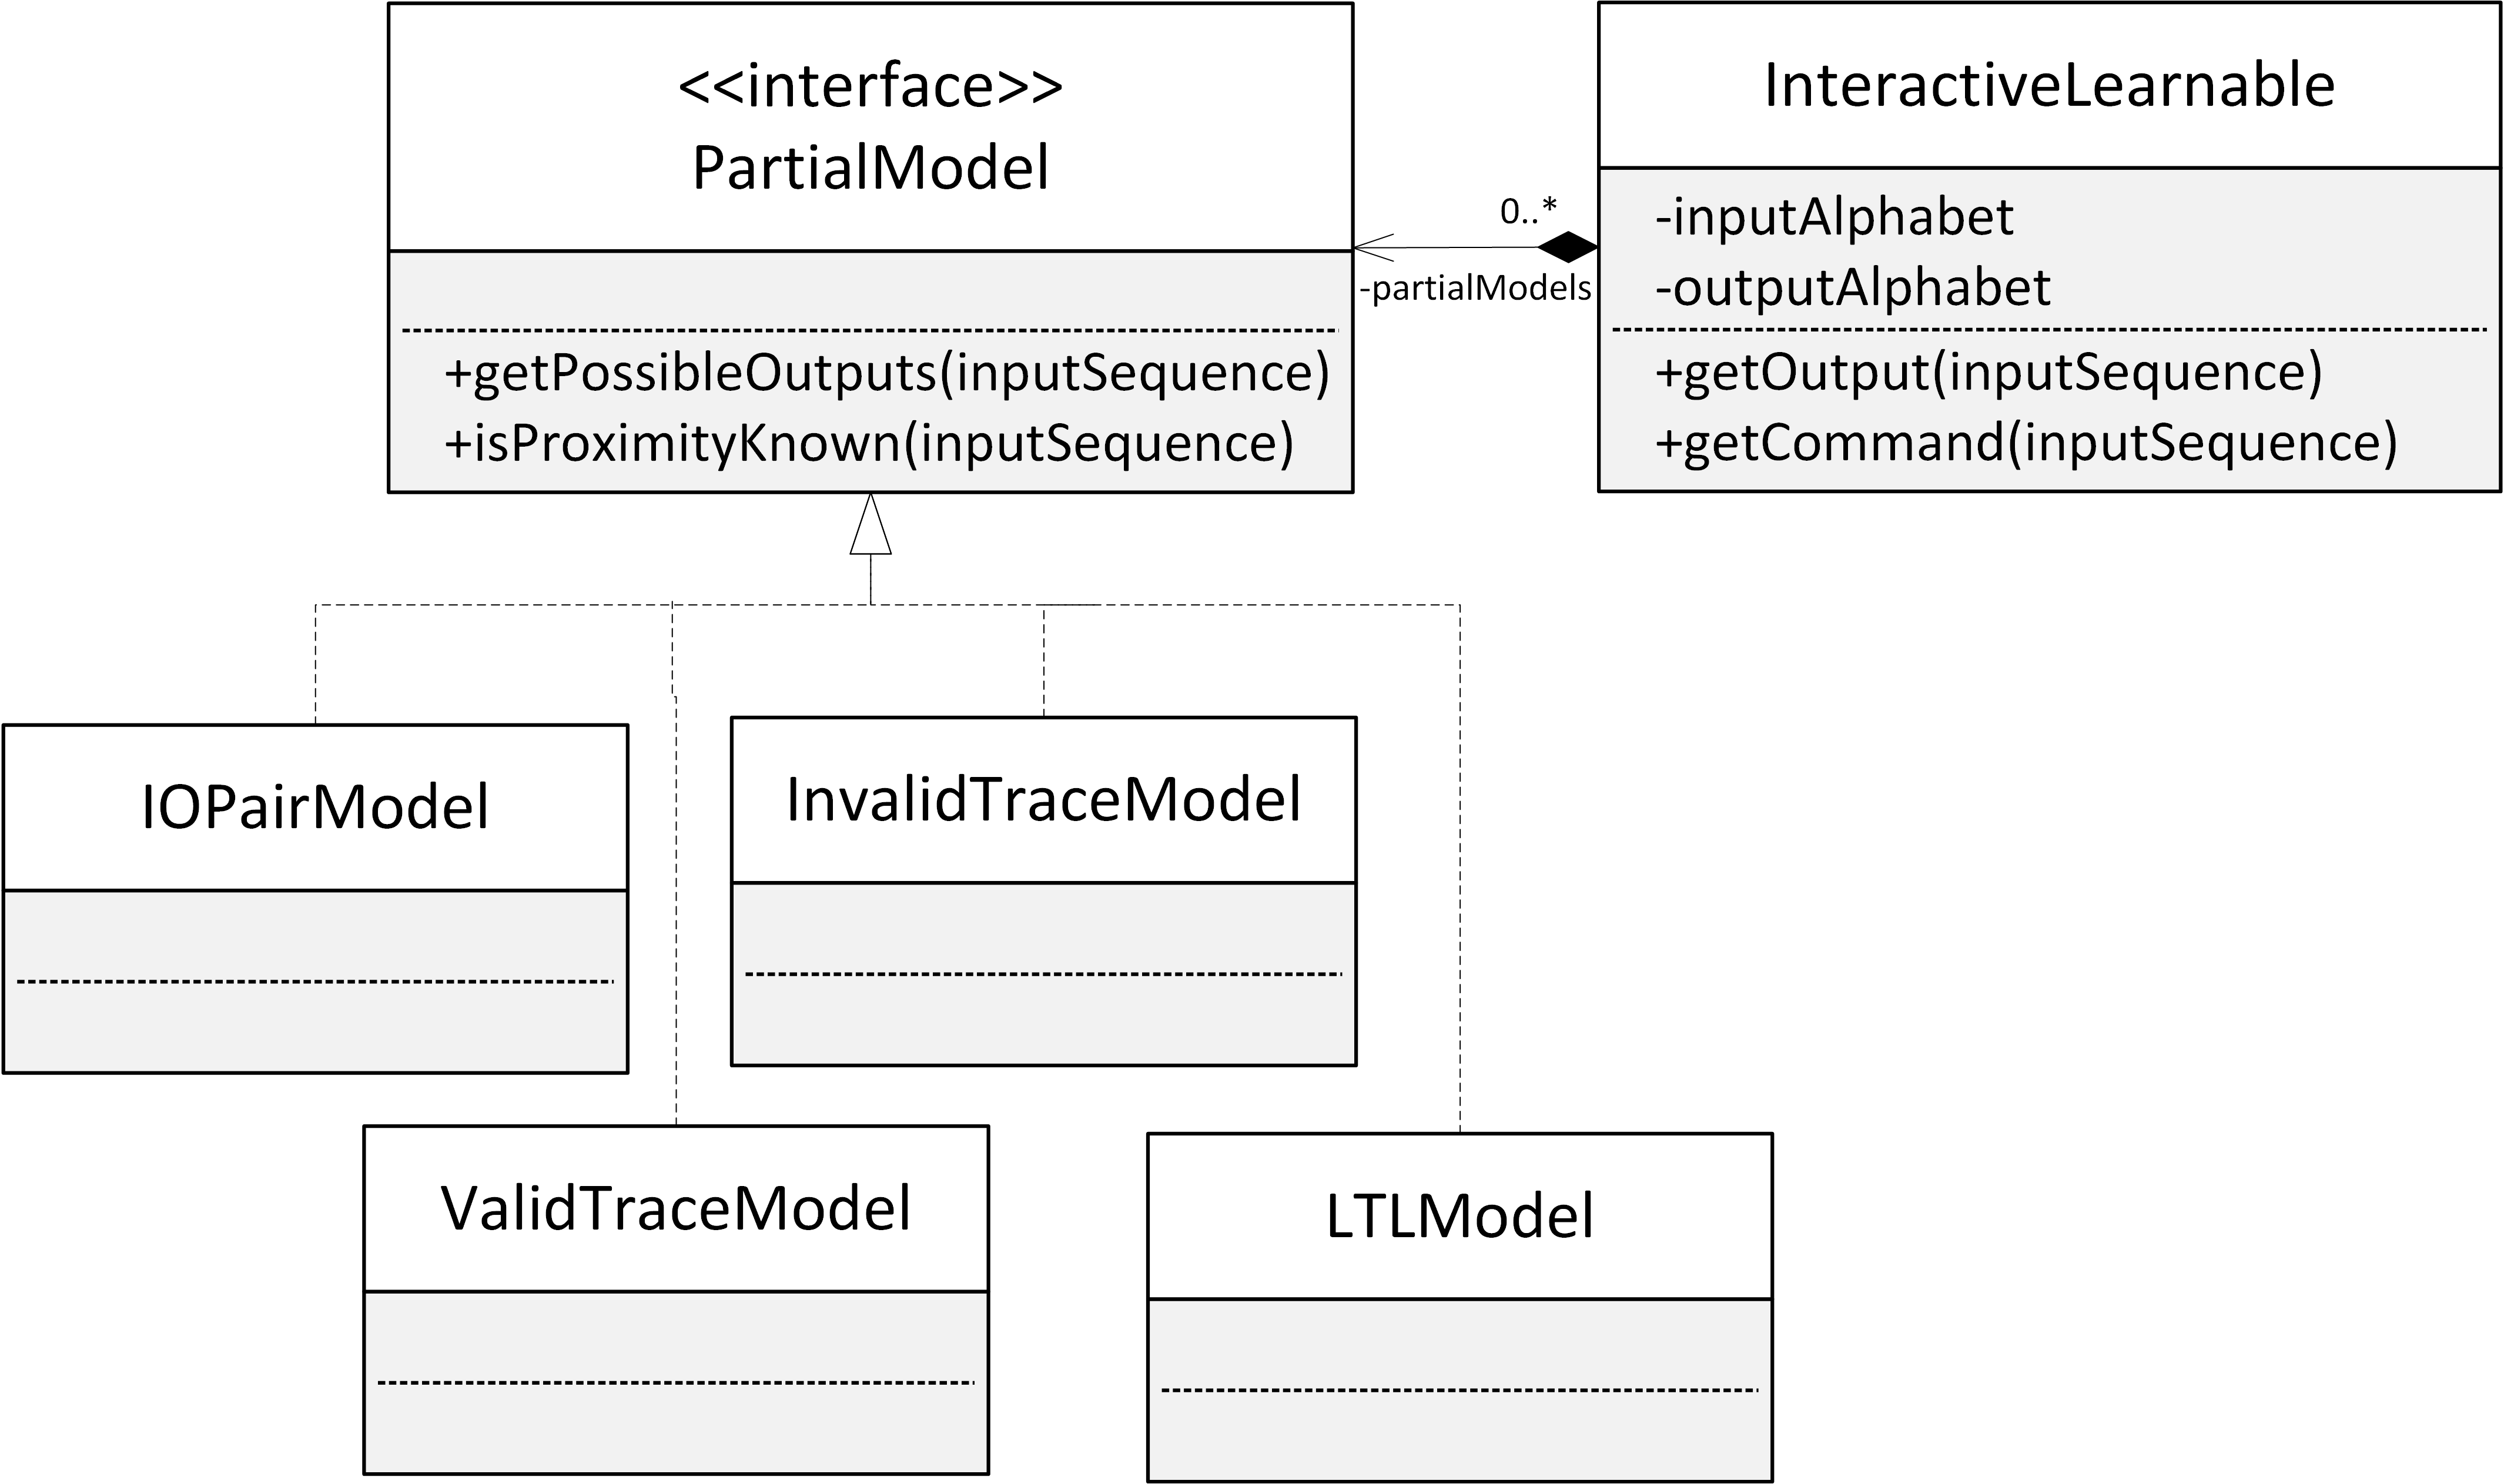
\includegraphics[width=150mm, keepaspectratio]{figures/architecture_interactivelearnable.png}
	%}
	\caption{Architecture of the interactive learnable component} 
	\label{fig_architcture_interactivelearnable}
\end{figure}

%---------------------------------------------------------------
\subsection{Trace-Based Models} \label{subs_traceintheframework}
%---------------------------------------------------------------
%TODO 
(hogyan működnek)
%---------------------------------------------------------------
\subsection{LTL Models} \label{subs_ltlintheframework}
%---------------------------------------------------------------
%TODO 
(hogyan lesznek használhatóak és hogyan működnek)

%---------------------------------------------------------------
\subsection{The Underlying Algorithm} \label{subs_dhcintheframework}
%---------------------------------------------------------------
In order to modify and optimize the learning, we built upon and designed a variant of the Direct Hypothesis Construction algorithm. The DHC algorithm learns through rounds of hypothesis creation, in which every round starts from the ground-up. This approach has the benefit of allowing the system under learning to behaviorally change through the run of the algorithm, and - in the case of interactive learning - allows the designing engineer(s) to add, remove and modify requirements as they please.

%---------------------------------------------------------------
\subsection{Caching} \label{subs_cachingintheframework}
%---------------------------------------------------------------
Caching the previous answers to queries can be a straightforward way of reducing the number of questions the user has to answer, specifically in the case of the DHC algorithm, where each learning round makes every single query that the previous did. Thus we propose a caching layer between the oracle and the learning algorithm, as seen in Figure [TODO], which controls which questions are forwarded to the oracle, and conversely, which can be automatically answered.

[TODO: ÁBRA]
%TODO: az oracle kérdezése költséges, így minél kevesebbszer akarjuk kérdezni
%---------------------------------------------------------------
\subsection{The Cost of Exploration (Command Handling)} \label{subs_commandhandling}
%---------------------------------------------------------------
(egyéb cím ötletek: a könnyen felfedezhető részek nyilvántartása, controlling the design space exploration, design space optimization, knowing what is unknown, reducing the cost of exploration, controlling design space partitions, abstract space partitioning, concept class)
%TODO: a költség az, hogy hányszor kérdezzük a usert, ezt akarjuk csökkenteni. Így nyilvántartjuk, hogy merre tudunk még információt kinyerni a már meglévő modellekből, csak azután megyünk a felhasználóhoz.

Active learning algorithms, and specifically in this case, the Direct Hypothesis Construction algorithm assume that the information they require are readily available, and thus follow a "greedy" approach of querying. While this is appropriate for automated solutions, greedily exploring the design space can result in several magnitudes larger amount of new, previously unexplored queries. The result of this is longer learning rounds (with more membership queries) exploring a larger amount of the behavior, and conversely less equivalence queries. To allow the designing engineer to more frequently validate the hypothesized model, and the control of which unexplored behavior should be explored, a less greedy approach would be necessary.

To solve the above issue, we introduce the concept of adaptive active automaton learning, which uses behavioral types - as illustrated in Figure \ref{fig_architcture_commandhandling} - as a heuristic to adaptively decide if and where a greedy approach should be taken. Already explored behaviors (e.g. previously queried, cached) as well as easily explorable ones (e.g. which can be inferred from some already provided requirement)  can be answered in an automated way, allowing greediness. On the other hand, completely unknown behaviors should be explored in a more reserved manner, controlled by the user - not the automaton learning algorithm.

\begin{figure}[!ht] 
	\centering
	\fbox{
	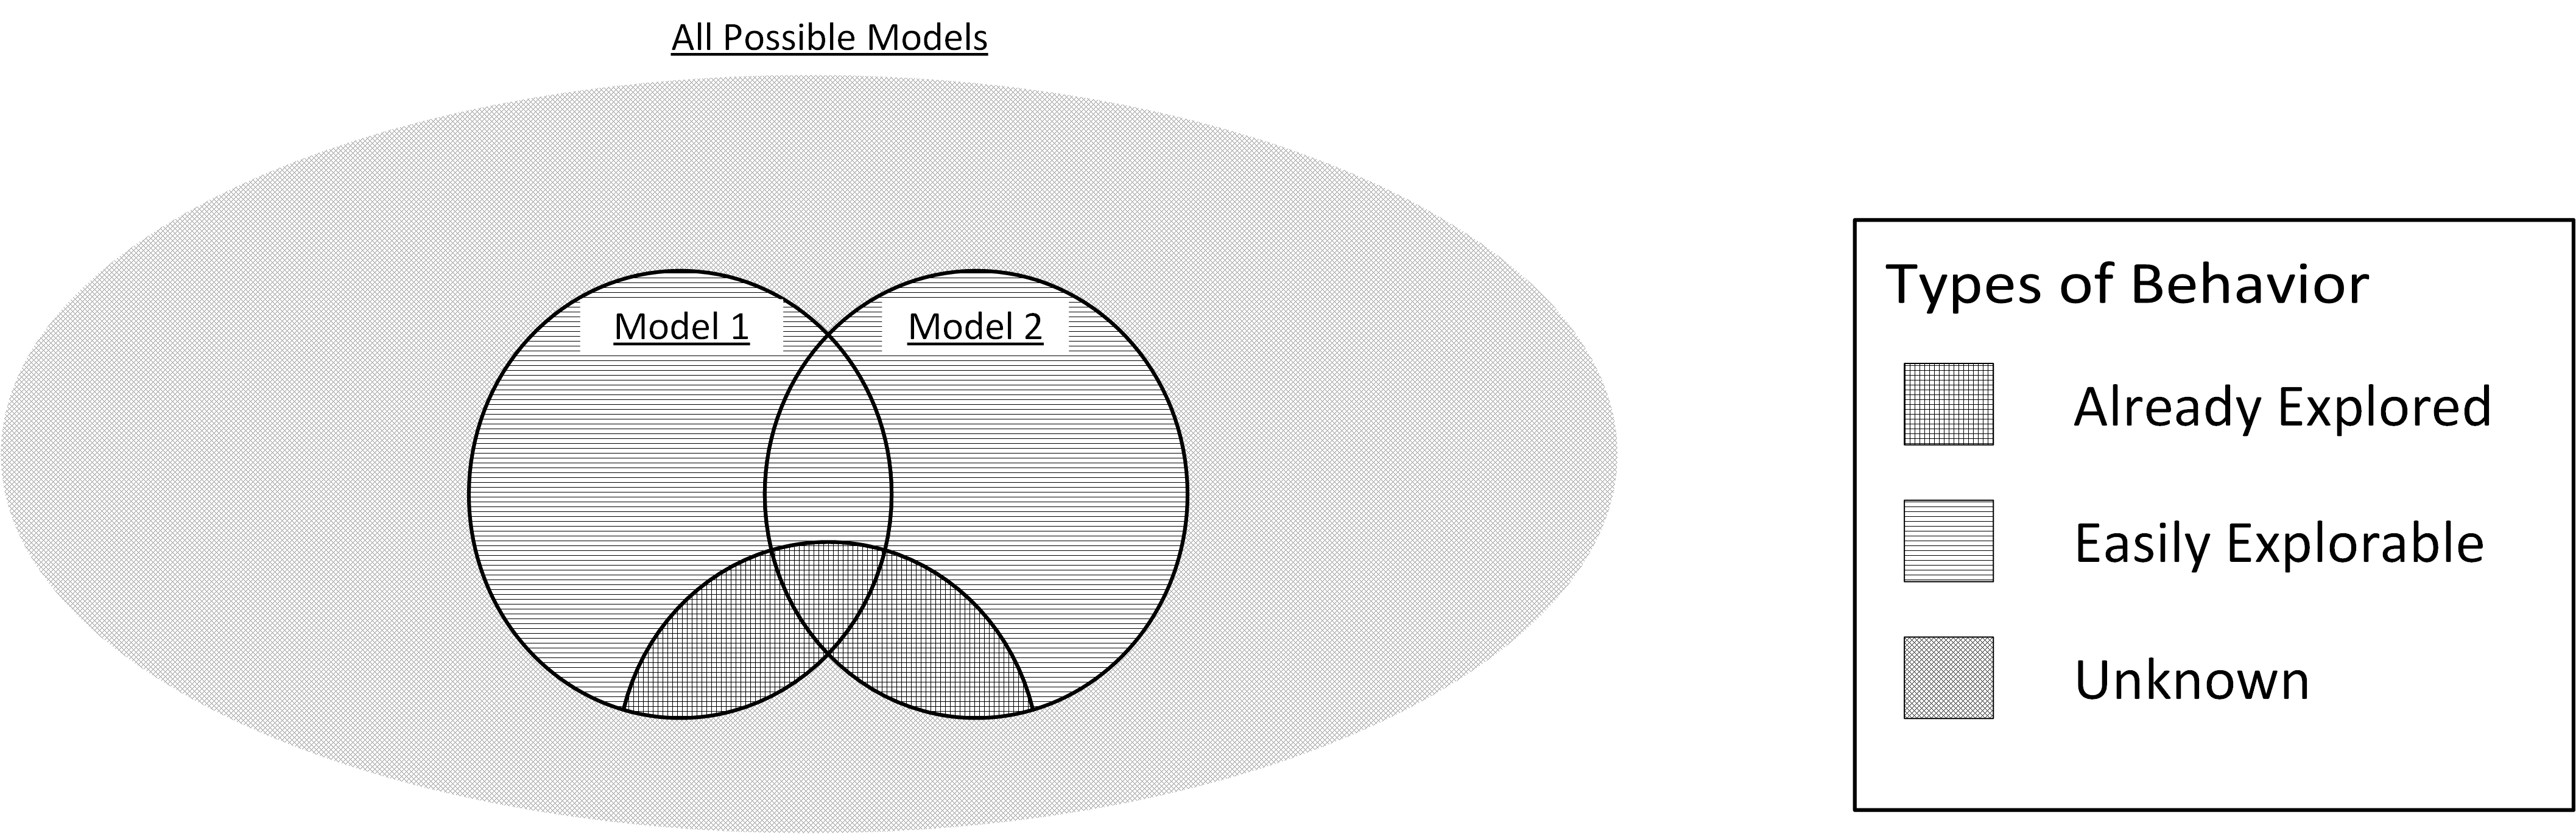
\includegraphics[width=150mm, keepaspectratio]{figures/architecture_commandhandling.png}
	}
	\caption{Types of behavior during the learning process} 
	\label{fig_architcture_commandhandling}
\end{figure} %TODO

%---------------------------------------------------------------
\subsection{Automata Minimization} \label{subs_minimizationintheframework}
%---------------------------------------------------------------
(per round vs per learning)
%TODO

